\documentclass[UTF8]{ctexart}

\usepackage{subfiles}  

%下面的语句, 引入你的头部设置文件
\usepackage{C:/phpStorm_proj/02_myself_ID_EGO/+100_latex_all_math_sel/myPreamble} 
%必须是绝对路径,才能让各个tex在单独编译时使用到

\title{文件名}


%---------------------------------


\begin{document}
	\tableofcontents % 生成目录
	\date{} % 若不写这句, 则默认也会渲染出日期, 所以我们要手动赋空值
	\maketitle  %这行代码, 让你前面的 title, author, date生效
	
		
	\part{中心极限定理 central limit theorem}
		
		
	\section{``中心极限定理"说的是什么?}
	``中心极限定理"有好几种不同的表述方式, 但其核心的数学性质只有一条 ---  \textbf{大量``独立"的随机变量相加, 无论这些各随机变量的``本身分布"是怎样的,它们相加后的结果, 必定会趋向于"正态分布".} 换言之, 这就意味着 --- 正态分布是必然产生的. \\
	
	\textbf{中心极限定理告诉我们 : 只要随机事件A, 是由很多``相互独立(而互不影响)的因素"共同起作用而决定的, 则无论每个因素本身是什么分布, 这个随机事件A, 最终都会形成``正态分布".} \\
	
	比如: \\
	- 影响人身高的因素很多,营养、遗传、环境、族裔、性别等都有影响, 这些因素的综合效果, 就会使人的身高, 服从正态分布. \\
	- 同样, 影响考试成绩的因素也很多,自身的能力、家庭教育、智商、专注力, 考前的情绪、身体状况等也都有影响. 这些因素互相独立. 但当这些影响因素加总在一起后, 对考试成绩的整体影响 --- 即考试的分数结果, 就会服从``正态分布". \\
	
	所以, 我们现在就明白了 : 世界上为什么会有这么多事情, 都服从``正态分布"? 就是因为很多事情, 都是由多个``独立"的随机因素, 共同起作用后的结果. \\
	
	因为\textbf{任何分布叠加, 最终都会形成正态分布},所以无论是``对数分布"还是``幂律分布",无论是``指数分布"还是其他什么分布,只要自身不断演化,不断自己叠加自己,最终也一样会变成正态分布. 所以\textbf{我们可以这么说,所有的分布,不是``正态分布", 就是在变成``正态分布"的路上.} \\	
	所以, ``中心极限定理"是因,``正态分布"是果. \textbf{正因为这个宇宙中有``中心极限定理"存在,所以才会推导出``正态分布".} \\
	
	当然, 现实世界里,影响一个随机事件的各种因素,不可能完全是理想状态下的``相互独立",而是会互相影响的. 所以, 我们身边依然存在各种各样的其他分布. \\
	
	
	
	
	
	\section{大量``n重伯努利试验"的结果, 就能产生``正态分布"的概率函数曲线}
	
	\begin{myEnvSample}
		比如, 抛硬币(以连续抛10次硬币, 为一次(一组)试验). 下面图中, 白色代表``得到正面", 黑色代表``得到反面". \\
		- 第一次(组)试验, 得到结果: 7正, 3反. \\
		- 第一次(组)试验, 得到结果: 9正, 1反. \\
		- ... \\
		
		进行100次(组)试验后,  得到100个结果. \\
		
		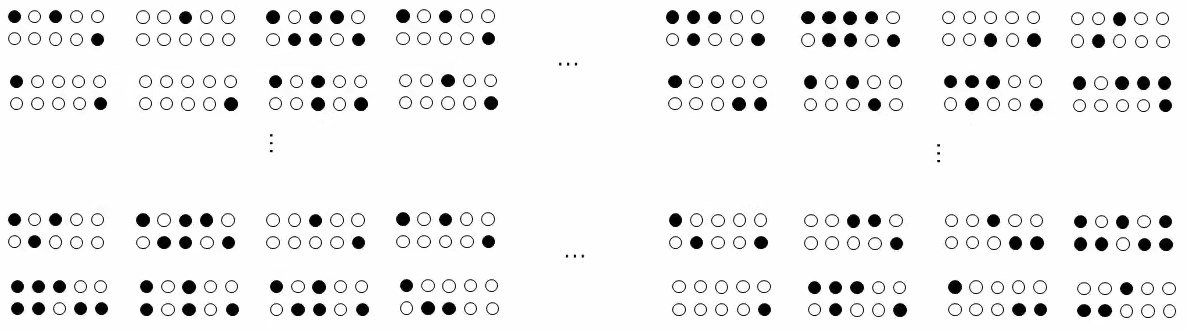
\includegraphics[width=1\textwidth]{/0199.png} \\
		
		把每组试验的结果中的``正面朝上"数量, 记下来, 分别是: 7,9,4,..., 共100个数据. \\
		然后, 统计这100个数据里面, 有多少个``正面数量是1"的; 有多少个``正面数量是2"的, ..., 统计在直方图上. \\
		
		研究任何统计数据,核心工具都是``直方图(Histogram)". 直方图能让我们了解``数据集的分布情况". \\
		
		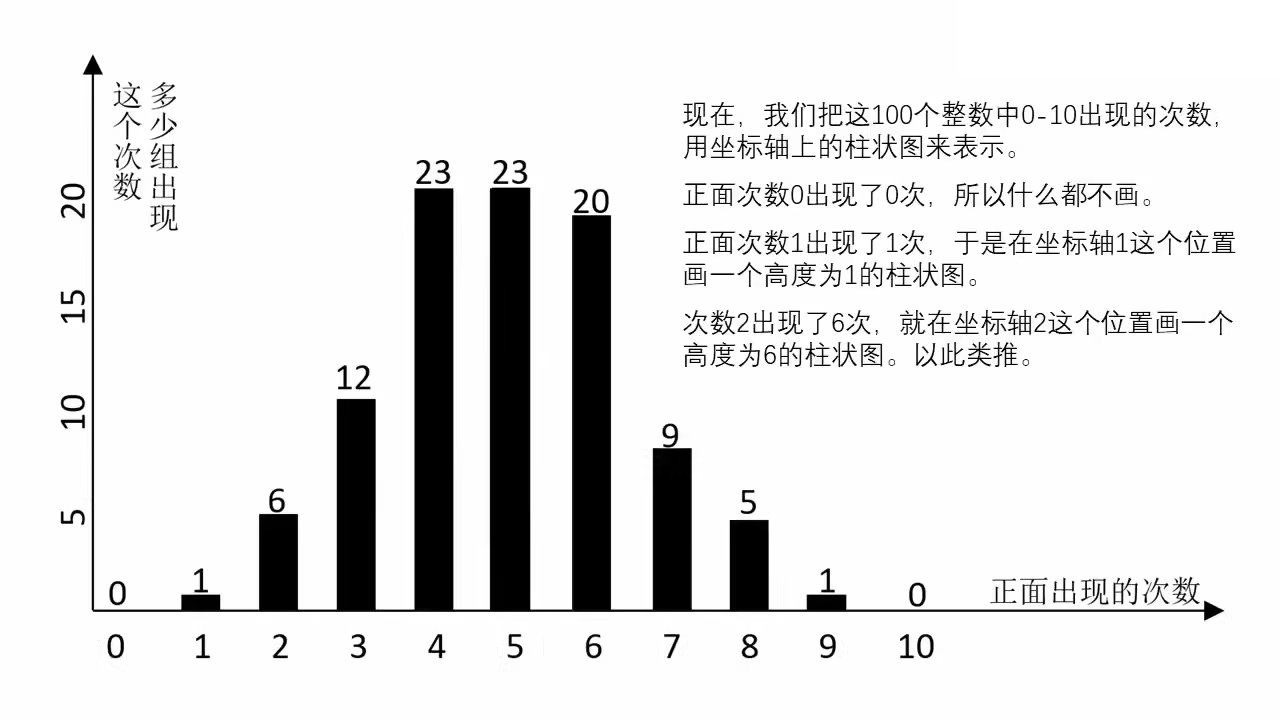
\includegraphics[width=0.8\textwidth]{/0200.png} \\
		
		我们可以发现, 它呈现出``正态分布"的钟形曲线形状. \\
		
		其实. \textbf{抛一次硬币试验, 它属于``伯努利试验". 抛10次硬币, 叫做``10重伯努利试验".} \\
		\textbf{我们进行100组这样的试验, 就叫做``100次 10重伯努利试验".} \\
		统计结果表明, \textbf{大量的``n重伯努利试验"的结果, 能产生``正态分布"曲线.} 	
	\end{myEnvSample}
	\vspace{1em} 
	
	
	
	\begin{myEnvSample}
		其实, 我们可以用一种更简单的方法, 来模拟``n重伯努利试验". --- Galton knocked boards 高尔顿钉板. \\
		
		顶端的珠子往下落, 遇到钉子时, ``往左"或``往右"落下的概率, 各是0.5. 这就可以看做``抛了一次硬币". 珠子向左, 可以看成``硬币正面朝上"; 向右, 可以看成``反面朝上". \\
		
		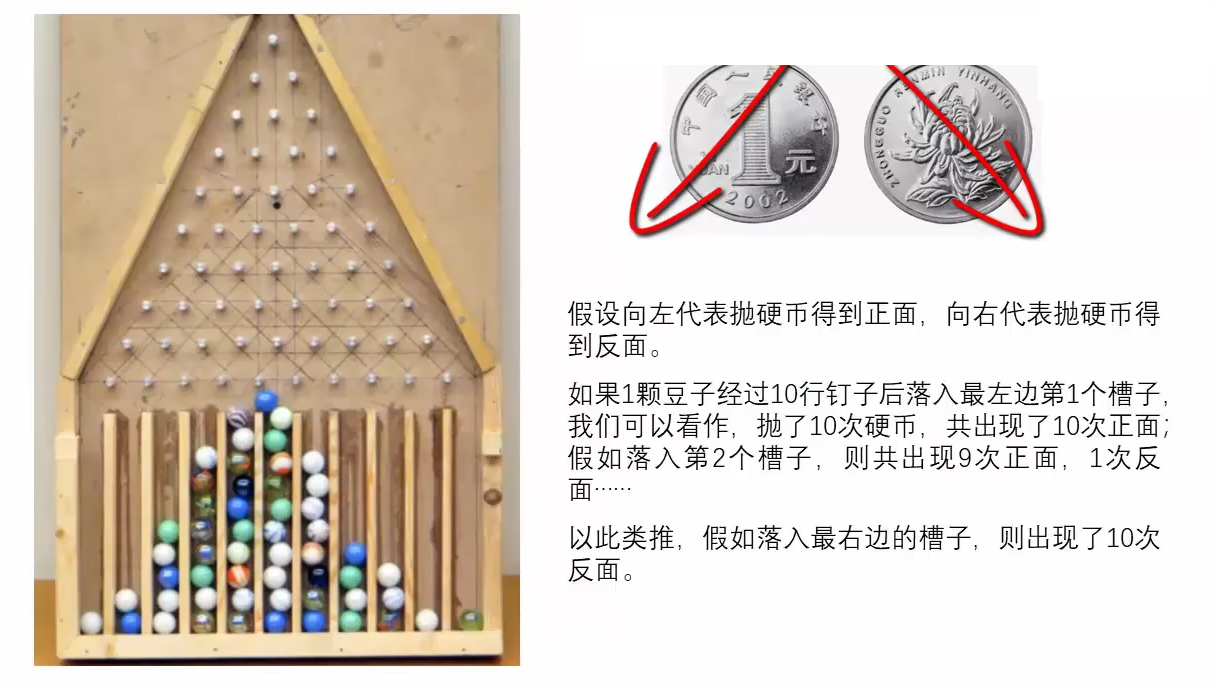
\includegraphics[width=0.9\textwidth]{/0201.png} \\
				
		假设我们有10行钉子, 下方的槽就会有11个. \textbf{我们可以根据珠子落入哪个槽, 来判断它经过10行钉子时, 经历了几次向左, 几次向右.} \\
		- 比如, 假如1颗珠子落入中间的槽, 那么它肯定是经过了5次向左, 5次向右. \\
		- 如果1颗珠子, 经过10行钉子后, 落入最左边第1个槽, 我们就可以看做是: 抛了10次硬币, 共出现10次正面(珠子10次向左). \\
		- 如果落入第2个槽, 就可看做: 出现9次正面, 1次反面. \\
		同理, 假如落在最右边的槽, 就可看做: 出现了10次反面. \\
		
		即: 从``最上"落到``最下面"的路径走一次, 就相当于做了一组(10次的``得到正面或反面"的抛硬币)试验. \\
		在每一行钉子处(往左还是往右), 就代表做一次抛硬币试验(伯努利试验). \\
		所以一条路径, 代表``做了1次 10重伯努利试验". \\
		100颗钉子落下来(走100条路径), 就代表做了``100次 10重伯努利试验". \\		
		
		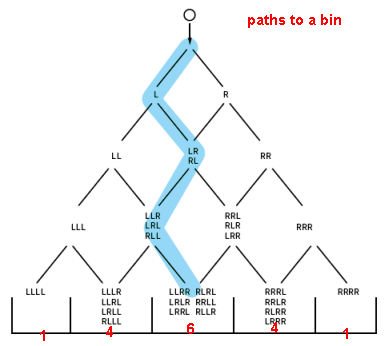
\includegraphics[width=0.5\textwidth]{/0204.png} \\
		
		10行钉子, 得到的这个正态分布曲线, 还不够光滑. 这是因为我们只放了100颗珠子, 规律表现得还不够明显. \\
		我们放1000颗珠子, 经过10行钉子, 得到的正态曲线, 就会更光滑. 这说明: \textbf{重复试验次数越多, 我们观察到的规律性就越强.} \\
		
		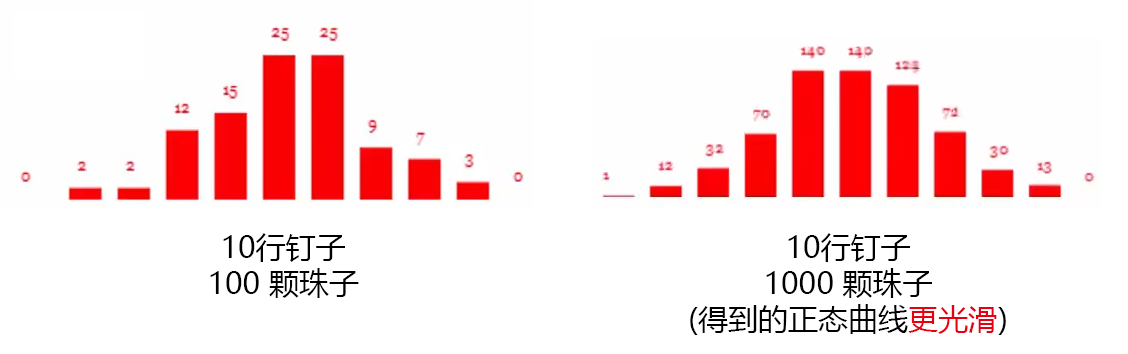
\includegraphics[width=0.8\textwidth]{/0202.png} \\		
		
		
		下面, 我们把钉子的行数, 从 n=10行, 加大到 n=20行. 再来看1000个珠子的下落结果. \\
		- 钉子行数n越多, 下面的槽数就更多, 正态分布曲线越矮胖 (即其方差$\sigma^2$越大).  \\		
		- 钉子行数n越少, 下面的槽数就越少, 珠子就只能落在这更少数量的槽里面, 正态分布曲线越高瘦 (即其方差越小).  \\		
		
		
		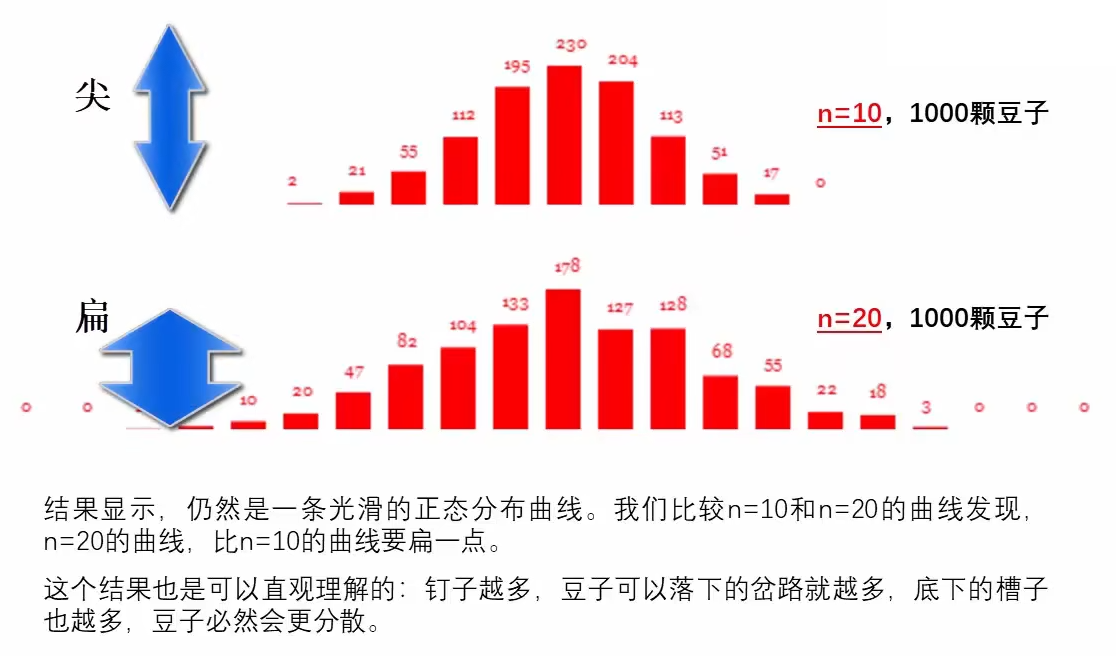
\includegraphics[width=0.8\textwidth]{/0203.png} 	
		\end{myEnvSample}
	\vspace{1em} 
	
	
	
	
	
	\begin{myEnvSample}
		如果上例的高尔顿钉板, \textbf{在每行的钉子处, 向左或向右的概率不同, 结果会怎样呢? 结果依然会得到``正态分布".}   \\
		我们重复做4次上述试验, 结果显示, 分布依然是正态分布. \textbf{只不过每次曲线的对称轴$\mu$的位置有所不同.} \\
		
		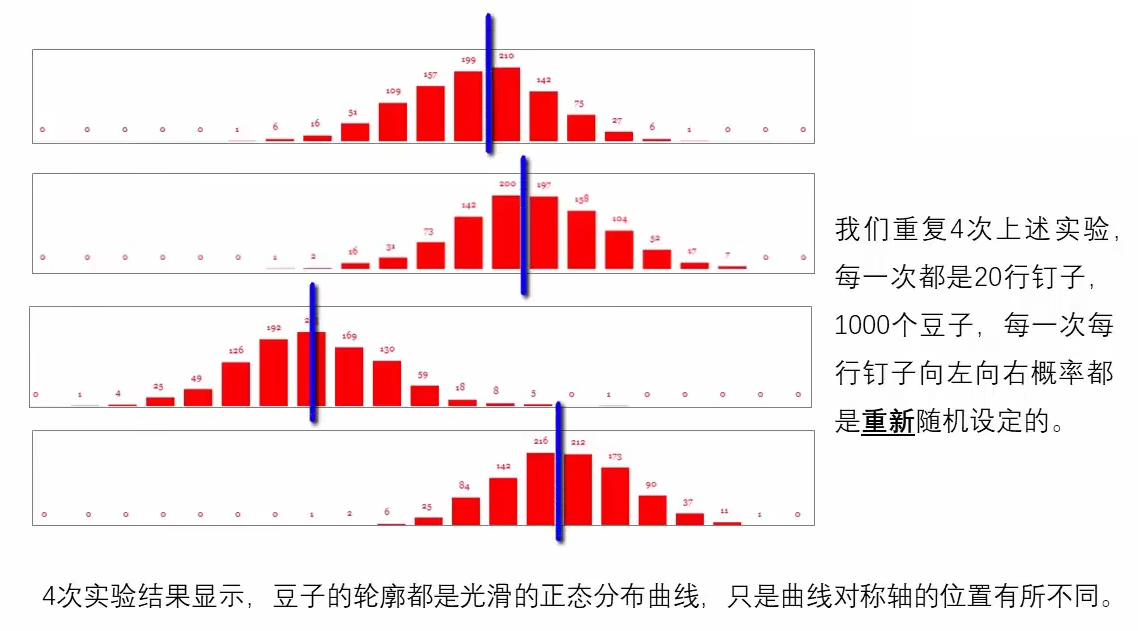
\includegraphics[width=0.8\textwidth]{/0205.png} 	\\
		
		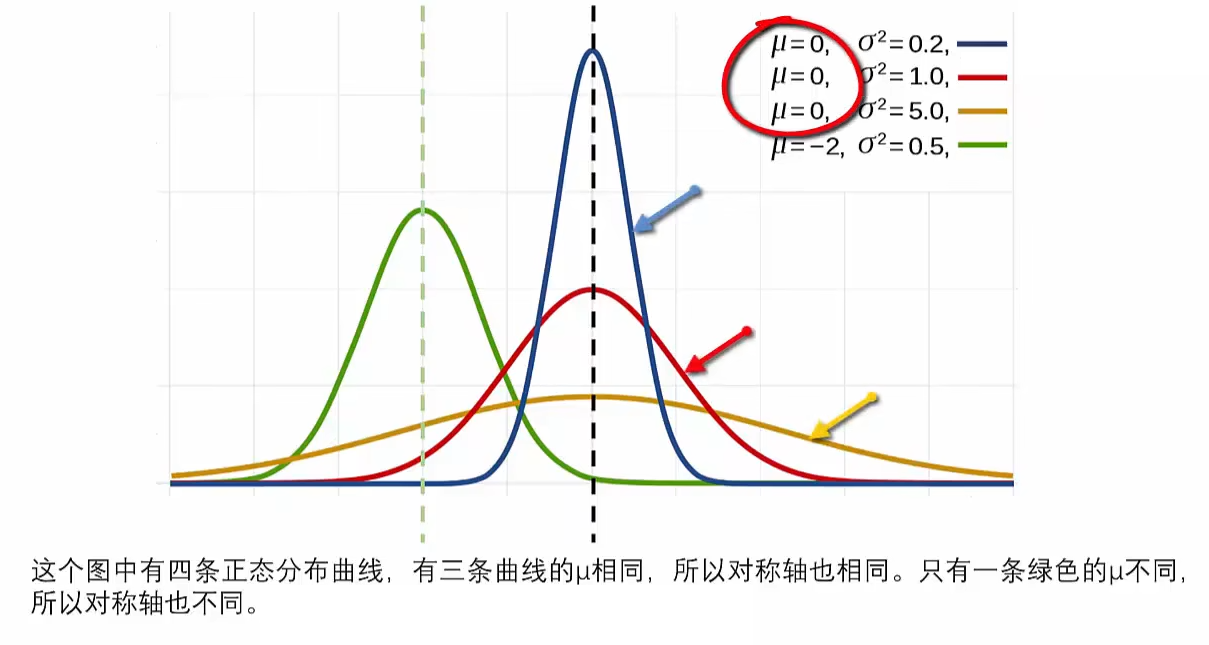
\includegraphics[width=0.8\textwidth]{/0206.png} 
	\end{myEnvSample}


	中心极限定理, 就是说 : 如果一个结果是由大量的不相干的因素, 累加导致的,那么其总合的结果, 一定表现为``正态分布". \\
	
	例如, 一个考生的高考英语成绩, 受到了无数(相关或不相关的)因素的影响. 每一个因素,都可能使最终英语分数更高一点,或者更低一点. \\
	每个独立因素对成绩所产生的影响, 就好比一颗豆子经过一颗钉子时,向左向右的概率说不清楚, 但这个概率一般不会是左右各0.5. \\	
	在无数因素影响后, 最终得到了一个高考英语成绩, 就相当于一颗豆子经过了无数行钉子的下落,最终尘埃落定,落到槽子里. \\
	
	数十万计考生最后的成绩分布,相当于数十万个豆子,经过了无数行钉子落到槽子里. 根据``中心极限定理", 其分布必然是``正态分布". \\
	考最高分的人,和考最低分的人,必然都只占少数,都分布在曲线两边的尾巴上(因为一颗豆子,\textbf{要想从一开始就一路向左,或一路向右落到槽子里,太难了}). 而大多数人,必然都是在中间位置,考一个不高不低的分数. \\
	
	
	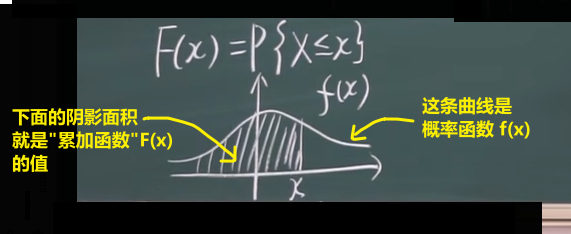
\includegraphics[width=0.8\textwidth]{/0208.png} 
	
	
	
	\section{正态分布是这个宇宙的归宿}
	
	信息论领域中, 发现了``嫡最大原理”. 也就是说, \textbf{在一个孤立系统中,嫡总是在不断增大. 而``正态分布", 是所有已知均值($\mu$)和方差($\sigma^2$)的分布中,信息嫡最大的一种分布.} 这就意味着: 如果``嫡不断增长"是孤立系统确定的演化方向,那嫡的最大化,也就是``正态分布",就是孤立系统演化的最终必然结果了.
	
	
	
	
	
	\section{当我们不知道某个随机事件, 服从什么分布的时候, 就先假设它服从``正态分布", 然后再用实际数据来验证.}
	
	为什么要先假设它(可能会)服从``正态分布"呢? 因为: \\
	- 这个世界中, ``正态分布"太常见了,所以假设一个随机事件是服从``正态分布"的, 要比假设它服从其他分布, 成功概率更高. \\
	- 如果我们事后的验证后发现,这个\textbf{随机事件不服从``正态分布",}那么我们就知道 : \textbf{它一定不满足正态分布背后的"中心极限定理".} 进一步, \textbf{既然它不满足``中心极限定理", 那么原因就会是 --- 要么是它的``独立影响因素"数量不够多; 要么是各种影响因素``不相互独立"; 要么是某种影响因素的影响力太大了等等}... 这些合理的推断, 就为我们接下来的研究, 指明了方向. \\
	
	
	
	
	
	
	
	
	
	
	
	
\end{document}